\documentclass[aspectratio=169,10pt]{beamer}

% Theme selection & aesthetic color scheme
\usetheme{Madrid}
\usecolortheme{whale}

% Typography & Math
\usepackage[utf8]{inputenc}
\usepackage{helvet}
\usepackage{booktabs}
\usepackage{listings}
\usepackage{xcolor}
\usepackage{tikz}
\usetikzlibrary{shapes.geometric, arrows.meta, positioning, calc, backgrounds}

% Custom modern palette
\definecolor{NavyBlue}{RGB}{26, 42, 58}
\definecolor{TealAccent}{RGB}{0, 150, 136}
\definecolor{SlateGray}{RGB}{84, 110, 122}
\definecolor{LightBg}{RGB}{245, 247, 250}
\definecolor{CodeBg}{RGB}{30, 30, 30}
\definecolor{CardBorder}{RGB}{207, 216, 220}

% Beamer color overrides
\setbeamercolor{palette primary}{bg=NavyBlue,fg=white}
\setbeamercolor{palette secondary}{bg=SlateGray,fg=white}
\setbeamercolor{palette tertiary}{bg=TealAccent,fg=white}
\setbeamercolor{structure}{fg=NavyBlue}
\setbeamercolor{frametitle}{bg=NavyBlue,fg=white}
\setbeamercolor{title}{bg=NavyBlue,fg=white}
\setbeamercolor{block title}{bg=NavyBlue,fg=white}
\setbeamercolor{block body}{bg=LightBg,fg=black}
\setbeamercolor{block title example}{bg=TealAccent,fg=white}
\setbeamercolor{block body example}{bg=LightBg,fg=black}

% Remove default navigation symbols
\setbeamertemplate{navigation symbols}{}

% Listings configuration for Java code
\lstset{
    language=Java,
    basicstyle=\ttfamily\scriptsize\color{white},
    backgroundcolor=\color{CodeBg},
    keywordstyle=\color{cyan}\bfseries,
    stringstyle=\color{orange},
    commentstyle=\color{green!70!white}\itshape,
    numberstyle=\tiny\color{gray},
    numbers=none,
    breaklines=true,
    showstringspaces=false,
    tabsize=2,
    frame=single,
    rulecolor=\color{SlateGray}
}

% Title, Author & Metadata
\title[Fleet \& Car Rental System]{Automated Vehicle Fleet \& Car Rental Management System}
\subtitle{Comprehensive Desktop Application Implementing Units 1 to 5 of Java OOP}
\author[Aarush Dubey]{Aarush Dubey}
\institute[SRM University AP]{Department of Computer Science and Engineering\\SRM University AP}
\date{\today}

\begin{document}

% -------------------------------------------------------------
% SLIDE 1: Title Slide
% -------------------------------------------------------------
\begin{frame}
    \titlepage
\end{frame}

% -------------------------------------------------------------
% SLIDE 2: Project Architecture (3-Tier)
% -------------------------------------------------------------
\begin{frame}{System Architecture \& High-Level Flow}
    \begin{columns}[T]
        \begin{column}{0.48\textwidth}
            \begin{block}{Architectural Overview}
                \small
                \begin{itemize}
                    \item \textbf{Single-File Engineering}: All tiers encapsulated in \texttt{Main.java} for clean portability.
                    \item \textbf{Decoupled Layers}: GUI layer communicates via event handlers with business logic; persistence is managed by JDBC.
                    \item \textbf{Autonomous Execution}: Self-initializes SQLite database table (\texttt{vehicles}) and seeds demo records.
                \end{itemize}
            \end{block}
            \begin{exampleblock}{Key Architectural Goals}
                \small
                $\bullet$ Zero external server dependencies (Embedded SQLite).\\
                $\bullet$ Native cross-platform desktop UI (Java Swing).\\
                $\bullet$ Asynchronous non-blocking fleet dispatch.
            \end{exampleblock}
        \end{column}
        
        \begin{column}{0.48\textwidth}
            \centering
            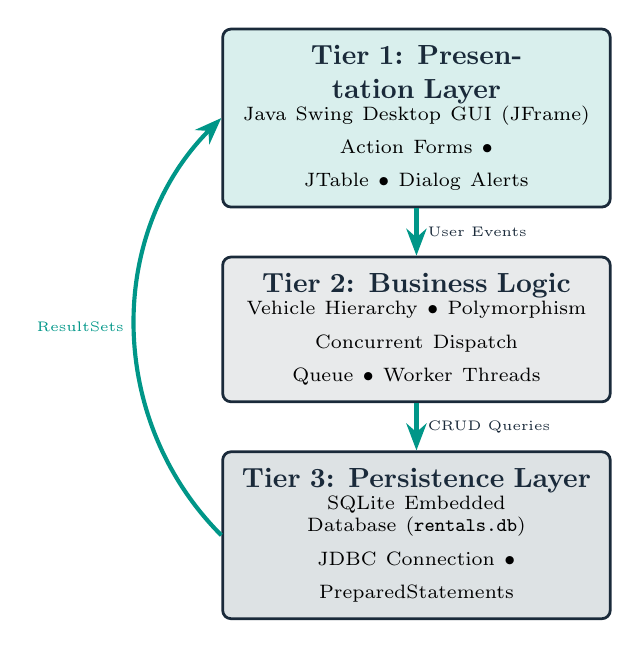
\begin{tikzpicture}[
                tier/.style={rectangle, draw=NavyBlue, fill=LightBg, rounded corners=3pt, text width=4.5cm, align=center, inner sep=6pt, line width=1pt},
                arrow/.style={-{Stealth[scale=1.0]}, line width=1.5pt, color=TealAccent}
            ]
                \node[tier, fill=TealAccent!15] (tier1) {
                    \textbf{\color{NavyBlue}Tier 1: Presentation Layer}\\
                    \scriptsize Java Swing Desktop GUI (JFrame)\\
                    Action Forms $\bullet$ JTable $\bullet$ Dialog Alerts
                };
                
                \node[tier, fill=NavyBlue!10, below=0.6cm of tier1] (tier2) {
                    \textbf{\color{NavyBlue}Tier 2: Business Logic}\\
                    \scriptsize Vehicle Hierarchy $\bullet$ Polymorphism\\
                    Concurrent Dispatch Queue $\bullet$ Worker Threads
                };
                
                \node[tier, fill=SlateGray!20, below=0.6cm of tier2] (tier3) {
                    \textbf{\color{NavyBlue}Tier 3: Persistence Layer}\\
                    \scriptsize SQLite Embedded Database (\texttt{rentals.db})\\
                    JDBC Connection $\bullet$ PreparedStatements
                };
                
                \draw[arrow] (tier1) -- node[right, font=\tiny, text=NavyBlue]{User Events} (tier2);
                \draw[arrow] (tier2) -- node[right, font=\tiny, text=NavyBlue]{CRUD Queries} (tier3);
                \draw[arrow] (tier3.west) to[bend left=45] node[left, font=\tiny, text=TealAccent]{ResultSets} (tier1.west);
            \end{tikzpicture}
        \end{column}
    \end{columns}
\end{frame}

% -------------------------------------------------------------
% SLIDE 3: Unit 1 - OOP Principles & UML Hierarchy
% -------------------------------------------------------------
\begin{frame}{Unit 1: Object-Oriented Programming \& Class Hierarchy}
    \begin{columns}[T]
        \begin{column}{0.48\textwidth}
            \begin{block}{OOP Fundamentals Applied}
                \small
                \begin{itemize}
                    \item \textbf{Abstraction}: Abstract base class \texttt{Vehicle} defines identity, base rate, and abstract \texttt{calculateRent(int days)}.
                    \item \textbf{Inheritance}: \texttt{Car}, \texttt{Bike}, and \texttt{Truck} extend \texttt{Vehicle} with specialized attributes.
                    \item \textbf{Polymorphism}: Dynamic method dispatch executes customized rental pricing logic per vehicle subclass at runtime.
                    \item \textbf{Encapsulation}: Private fields with validated public getters, setters, and status toggles.
                \end{itemize}
            \end{block}
        \end{column}
        
        \begin{column}{0.48\textwidth}
            \centering
            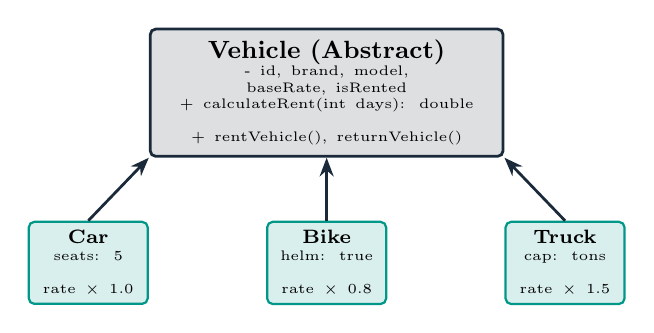
\begin{tikzpicture}[
                baseclass/.style={rectangle, draw=NavyBlue, fill=NavyBlue!15, rounded corners=2pt, text width=4.2cm, align=center, inner sep=4pt, line width=1pt},
                subclass/.style={rectangle, draw=TealAccent, fill=TealAccent!15, rounded corners=2pt, text width=1.3cm, align=center, inner sep=3pt, line width=0.8pt},
                arrow/.style={-{Stealth[scale=0.9]}, line width=1pt, color=NavyBlue}
            ]
                \node[baseclass] (base) {
                    \textbf{\small Vehicle (Abstract)}\\
                    \tiny - id, brand, model, baseRate, isRented\\
                    \tiny + calculateRent(int days): double\\
                    \tiny + rentVehicle(), returnVehicle()
                };
                
                \node[subclass, below left=0.8cm and 0.0cm of base] (car) {
                    \textbf{\scriptsize Car}\\
                    \tiny seats: 5\\
                    \tiny rate $\times$ 1.0
                };
                
                \node[subclass, below=0.8cm of base] (bike) {
                    \textbf{\scriptsize Bike}\\
                    \tiny helm: true\\
                    \tiny rate $\times$ 0.8
                };
                
                \node[subclass, below right=0.8cm and 0.0cm of base] (truck) {
                    \textbf{\scriptsize Truck}\\
                    \tiny cap: tons\\
                    \tiny rate $\times$ 1.5
                };
                
                \draw[arrow] (car.north) -- (base.south west);
                \draw[arrow] (bike.north) -- (base.south);
                \draw[arrow] (truck.north) -- (base.south east);
            \end{tikzpicture}
        \end{column}
    \end{columns}
\end{frame}

% -------------------------------------------------------------
% SLIDE 4: Unit 2 - Exception Handling & Robustness
% -------------------------------------------------------------
\begin{frame}[fragile]{Unit 2: Custom Exception Handling \& Defensive Design}
    \begin{columns}[T]
        \begin{column}{0.48\textwidth}
            \begin{block}{Defensive Architecture}
                \small
                \begin{itemize}
                    \item \textbf{Custom Exception}: \texttt{VehicleNotAvailableException} extends \texttt{Exception} to represent domain-specific booking conflicts.
                    \item \textbf{Checked Exception Paradigm}: Requires explicit handling via \texttt{try-catch} blocks or method declaration propagation (\texttt{throws}).
                    \item \textbf{Input Validation}: Protects against empty text fields, non-numeric price inputs, and unselected table rows before invoking the database.
                \end{itemize}
            \end{block}
        \end{column}
        
        \begin{column}{0.48\textwidth}
\begin{lstlisting}
// Domain Exception Definition
class VehicleNotAvailableException 
    extends Exception {
    public VehicleNotAvailableException(
        String message) {
        super(message);
    }
}

// Business Guard in Main.java
public void rentVehicle(String id) 
    throws VehicleNotAvailableException {
    Vehicle v = searchVehicle(id);
    if (v.isRented()) {
        throw new VehicleNotAvailableException(
            "Vehicle " + id + " is rented!");
    }
    v.setRented(true);
}
\end{lstlisting}
        \end{column}
    \end{columns}
\end{frame}

% -------------------------------------------------------------
% SLIDE 5: Unit 2 - Multithreading & Synchronization
% -------------------------------------------------------------
\begin{frame}{Unit 2: Multithreading, Queue Management \& Thread Safety}
    \begin{columns}[T]
        \begin{column}{0.48\textwidth}
            \begin{block}{Concurrency Design}
                \small
                \begin{itemize}
                    \item \textbf{UI Thread Responsiveness}: Heavy booking dispatch operations run on an asynchronous worker thread (\texttt{Thread}).
                    \item \textbf{Producer-Consumer Pattern}: Swing UI produces booking tasks; background daemon thread consumes tasks from queue.
                    \item \textbf{Thread Safety}: Synchronized blocks, \texttt{wait()}, and \texttt{notify()} coordinate access to the shared request list.
                \end{itemize}
            \end{block}
        \end{column}
        
        \begin{column}{0.48\textwidth}
            \centering
            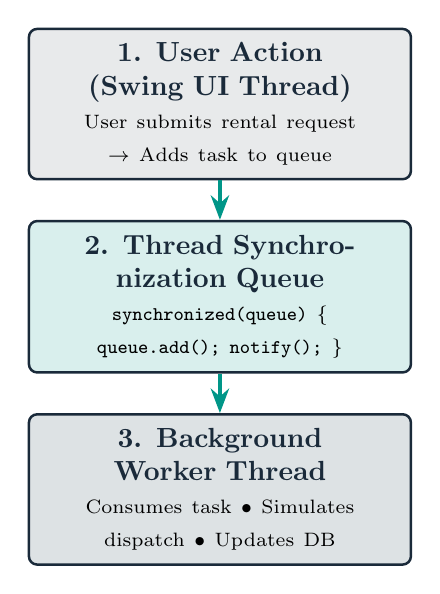
\begin{tikzpicture}[
                flowbox/.style={rectangle, draw=NavyBlue, fill=LightBg, rounded corners=3pt, text width=4.5cm, align=center, inner sep=5pt, line width=0.9pt},
                arrow/.style={-{Stealth[scale=1.0]}, line width=1.3pt, color=TealAccent}
            ]
                \node[flowbox, fill=NavyBlue!10] (ui) {
                    \textbf{\color{NavyBlue}1. User Action (Swing UI Thread)}\\
                    \scriptsize User submits rental request $\rightarrow$ Adds task to queue
                };
                
                \node[flowbox, fill=TealAccent!15, below=0.5cm of ui] (queue) {
                    \textbf{\color{NavyBlue}2. Thread Synchronization Queue}\\
                    \scriptsize \texttt{synchronized(queue) \{ queue.add(); notify(); \}}
                };
                
                \node[flowbox, fill=SlateGray!20, below=0.5cm of queue] (worker) {
                    \textbf{\color{NavyBlue}3. Background Worker Thread}\\
                    \scriptsize Consumes task $\bullet$ Simulates dispatch $\bullet$ Updates DB
                };
                
                \draw[arrow] (ui) -- (queue);
                \draw[arrow] (queue) -- (worker);
            \end{tikzpicture}
        \end{column}
    \end{columns}
\end{frame}

% -------------------------------------------------------------
% SLIDE 6: Unit 3 - Generics & Java Collections Framework
% -------------------------------------------------------------
\begin{frame}{Unit 3: Java Collections Framework \& Generic Storage}
    \begin{columns}[T]
        \begin{column}{0.48\textwidth}
            \begin{block}{Collection Mechanisms Applied}
                \small
                \begin{itemize}
                    \item \textbf{\texttt{ArrayList<Vehicle>}}: Dynamically stores active fleet members; provides ordered indexing for JTable rendering.
                    \item \textbf{\texttt{HashMap<String, Vehicle>}}: Key-value index mapping vehicle registration ID $\rightarrow$ vehicle object for $O(1)$ fast lookups.
                    \item \textbf{Generics Safety}: Strong type safety prevents runtime \texttt{ClassCastException} during vehicle queries.
                    \item \textbf{Iterators \& Streams}: Clean iteration over fleet inventory during status filtering and calculation passes.
                \end{itemize}
            \end{block}
        \end{column}
        
        \begin{column}{0.48\textwidth}
            \begin{exampleblock}{Collection Comparison in Project}
                \small
                \begin{tabular}{lll}
                    \toprule
                    \textbf{Data Structure} & \textbf{Time} & \textbf{Primary Purpose} \\
                    \midrule
                    \texttt{ArrayList<Vehicle>} & $O(n)$ & JTable UI binding \\
                    \texttt{HashMap<String, V>} & $O(1)$ & Instant ID search \\
                    \texttt{LinkedList<Request>} & $O(1)$ & Thread dispatch queue \\
                    \bottomrule
                \end{tabular}
            \end{exampleblock}
            \vspace{0.3cm}
            \begin{alertblock}{Design Benefit}
                \small
                Dual indexing provides fast user interface repainting while maintaining constant-time lookup performance during rentals.
            \end{alertblock}
        \end{column}
    \end{columns}
\end{frame}

% -------------------------------------------------------------
% SLIDE 7: Unit 4 - Java Swing GUI & Event Architecture
% -------------------------------------------------------------
\begin{frame}{Unit 4: Event-Driven Desktop GUI with Java Swing}
    \begin{columns}[T]
        \begin{column}{0.48\textwidth}
            \begin{block}{Swing GUI Components}
                \small
                \begin{itemize}
                    \item \textbf{Container Hierarchy}: \texttt{JFrame} host with \texttt{BorderLayout}, structured \texttt{JPanel} control ribbons, and a scrollable \texttt{JTable}.
                    \item \textbf{Interactive Controls}: \texttt{JTextField} inputs, \texttt{JComboBox} type selectors, and color-coded \texttt{JButton} actions.
                    \item \textbf{Event Delegation}: Decoupled \texttt{ActionListener} closures handle Add, Search, Rent, Return, and Delete events.
                    \item \textbf{Immediate Feedback}: Modal \texttt{JOptionPane} dialogs report success alerts and caught validation exceptions.
                \end{itemize}
            \end{block}
        \end{column}
        
        \begin{column}{0.48\textwidth}
            \centering
            \begin{tikzpicture}[
                guiframe/.style={rectangle, draw=NavyBlue, fill=LightBg, rounded corners=3pt, text width=4.8cm, inner sep=4pt, line width=1pt},
                panel/.style={rectangle, draw=SlateGray, fill=white, rounded corners=2pt, text width=4.4cm, inner sep=3pt}
            ]
                \node[guiframe] (frame) {
                    \textbf{\scriptsize Car Rental Management System (JFrame)}\\
                    \vspace{2pt}
                    \begin{tikzpicture}
                        \node[panel, fill=NavyBlue!10] (form) {
                            \tiny \textbf{Input Form}: ID, Brand, Model, Base Rate, Type\\
                            \tiny [Add Vehicle] \quad [Search] \quad [Update Rate]
                        };
                        \node[panel, fill=white, below=0.2cm of form] (table) {
                            \tiny \textbf{Live Fleet JTable} (Vehicle Data \& Status)\\
                            \tiny V001 | Toyota Camry  | \$50.0 | Available\\
                            \tiny V002 | Honda CBR     | \$30.0 | Rented\\
                            \tiny V003 | Ford F-150    | \$80.0 | Available
                        };
                        \node[panel, fill=TealAccent!15, below=0.2cm of table] (actions) {
                            \tiny \textbf{Operational Actions}: [Rent Selected] [Return Selected] [Delete]
                        };
                    \end{tikzpicture}
                };
            \end{tikzpicture}
        \end{column}
    \end{columns}
\end{frame}

% -------------------------------------------------------------
% SLIDE 8: Unit 5 - SQLite & JDBC Database Connectivity
% -------------------------------------------------------------
\begin{frame}[fragile]{Unit 5: Persistent Storage with SQLite \& JDBC}
    \begin{columns}[T]
        \begin{column}{0.48\textwidth}
            \begin{block}{Database Architecture}
                \small
                \begin{itemize}
                    \item \textbf{Embedded SQLite}: Zero configuration required; automatically creates and reads \texttt{rentals.db}.
                    \item \textbf{Connection Lifecycle}: Managed via \texttt{DriverManager.getConnection("jdbc:sqlite:rentals.db")}.
                    \item \textbf{SQL Injection Defense}: Parameterized queries via \texttt{PreparedStatement} ensure robust security.
                    \item \textbf{Full CRUD Support}: Create (Add), Read (Table Load), Update (Rate/Status), and Delete operations fully mapped.
                \end{itemize}
            \end{block}
        \end{column}
        
        \begin{column}{0.48\textwidth}
\begin{lstlisting}
// Parameterized SQL Statement Execution
String sql = "UPDATE vehicles SET daily_rate = ? " 
           + "WHERE vehicle_id = ?";

try (PreparedStatement pstmt = 
        conn.prepareStatement(sql)) {
    pstmt.setDouble(1, newDailyRate);
    pstmt.setString(2, vehicleId);
    pstmt.executeUpdate();
} catch (SQLException e) {
    System.err.println("DB Error: " + e.getMessage());
}
\end{lstlisting}
        \end{column}
    \end{columns}
\end{frame}

% -------------------------------------------------------------
% SLIDE 9: System Validation & Cross-Platform Execution
% -------------------------------------------------------------
\begin{frame}{System Validation, Testing \& Cross-Platform Verification}
    \begin{columns}[T]
        \begin{column}{0.55\textwidth}
            \begin{block}{Verification Matrix}
                \small
                \begin{tabular}{lll}
                    \toprule
                    \textbf{Feature / Subsystem} & \textbf{Test Mechanism} & \textbf{Status} \\
                    \midrule
                    SQLite Driver Loading & Static Initializer & Passed \\
                    Class Polymorphism & Pricing calculations & Passed \\
                    Exception Safeguards & Over-rental attempt & Caught \\
                    Thread Dispatch & Booking queue tests & Synchronized \\
                    Headless Environment & Terminal Fallback & Verified \\
                    macOS / Linux (.sh) & Bash compilation & Functional \\
                    Windows (.bat) & Batch compilation & Functional \\
                    \bottomrule
                \end{tabular}
            \end{block}
        \end{column}
        
        \begin{column}{0.41\textwidth}
            \begin{exampleblock}{One-Command Execution}
                \small
                \textbf{macOS / Linux}:
                \begin{itemize}
                    \item \texttt{./compile.sh}
                    \item \texttt{./run.sh}
                \end{itemize}
                \vspace{0.2cm}
                \textbf{Windows}:
                \begin{itemize}
                    \item \texttt{compile.bat}
                    \item \texttt{run.bat}
                \end{itemize}
            \end{exampleblock}
            \vspace{0.2cm}
            \begin{alertblock}{Headless Support}
                \scriptsize Automated check detects display servers; falls back cleanly to terminal output during continuous integration tests.
            \end{alertblock}
        \end{column}
    \end{columns}
\end{frame}

% -------------------------------------------------------------
% SLIDE 10: Conclusion & Viva Preparation
% -------------------------------------------------------------
\begin{frame}{Project Summary, Learning Outcomes \& Viva Q\&A}
    \begin{columns}[T]
        \begin{column}{0.48\textwidth}
            \begin{block}{Key Technical Takeaways}
                \small
                \begin{itemize}
                    \item \textbf{Unit 1}: Solid OOP modeling with clean polymorphism across specialized vehicle categories.
                    \item \textbf{Unit 2}: Defended against invalid states using custom exceptions and thread-safe queues.
                    \item \textbf{Unit 3}: High-performance data access using generic \texttt{ArrayList} and \texttt{HashMap}.
                    \item \textbf{Unit 4}: Intuitive, event-driven desktop GUI in pure Java Swing.
                    \item \textbf{Unit 5}: Reliable relational persistence with zero external setup using SQLite JDBC.
                \end{itemize}
            \end{block}
        \end{column}
        
        \begin{column}{0.48\textwidth}
            \begin{exampleblock}{Common Viva Questions Prepared}
                \small
                \begin{enumerate}
                    \item \textit{Why use abstract classes over interfaces?} $\rightarrow$ Common state retention (IDs, base rates).
                    \item \textit{Why PreparedStatement?} $\rightarrow$ Pre-compilation and SQL injection prevention.
                    \item \textit{How is thread safety guaranteed?} $\rightarrow$ Mutual exclusion on the shared booking queue.
                \end{enumerate}
            \end{exampleblock}
            
            \vspace{0.4cm}
            \centering
            \textbf{\Large Thank You!}\\
            \small Questions and Demonstrations Welcome.
        \end{column}
    \end{columns}
\end{frame}

\end{document}
